\section{Definitions}

%add refferences

%[REF] Survey of software refactoring tools \cite{erb2010survey}
This section presents some definitions regarding refactoring activities.

\subsection{Classification of the refactoring}
There are several levels of refactoring, a high level refactoring like design refactoring or a low level refactoring such as extract method refactoring operation. 
In between, exists combinational refactoring that is a combination of several low level refactoring operations.
The refactoring operations can also be classified by the effect that they have on software quality attributes, however that is a complex task to do. \cite{elish2011classification}

\subsection{Refactoring as a Process}
Refactoring can be done in two ways. %add citations
One is doing the refactoring in between programming and constantly performed. 
The other one is to do the refactoring as a different activity and done in bulks.
Regardless when is done, the refactoring can always be decomposed in this different activities: \cite{erb2010survey}

\begin{enumerate}
 \item Identify where to change the software
 \item Determine the adequate refactoring operation
 \item Have a way to protect the planned changes (e.g automated tests)
 \item Make the planned changes
 \item Access the refactoring benefits
 \item Maintain consistency between refactored and non-refactored code 
\end{enumerate}


%Eisenecker et al. [2000] defined requirements for the refactoring tools

%Functional requirements of a refactoring tools:
%Image, or explain in text => explain in text
%Non Functional requirements of a refactoring tool:
%Image. or explain in text.

\subsection{Refactoring Correctness}
%survey of software refactoring tools \cite{erb2010survey} %add citation
Refactoring must be correct and for some authors it means preserving the program behavior.
However there is no consensual definition for what behavior preservation is.
Some authors say that the behavior of the program is the output and preserving the output preserves the program behavior, but unfortunately that is not always true \cite{erb2010survey}.
For example in a class, if a method name is renamed and the program consists in printing that method name, by renaming that method the behavior of the program changes.

Another way do define it is to say that in order to preserve behavior it is needed to preserve the syntactic and semantic properties.
Preserving the syntactic properties is to preserve the syntax, and it is common sense that a refactoring should not invalidate a syntactic correct program.

Preserving the semantic of the program means to preserve the meaning of the program in the basic concept of the language. 
In other words, is to  maintain the semantic properties of all declarations after a refactoring and it should resolve to the same declarations they resolved before the refactoring operation.
Because preserving the syntax is easily seen, this document focus on the meaning-preservation of the refactoring operations. 


%suvey mens 2003 \cite{mens2003refactoring}
%What is behaviour and how to preserve it? 
%Observational behaviour, for the same input we get the same output, is not always sufficient.
%for example, for Real time systems it is important the time that a (sequence of) operations takes, for embedded systems it takes into account the memory and the power consumption and for safety-critical systems there is a defined safety that must be preserved. 
%In a theoretical world all this properties should be preserved by a refactoring, however in practice that is not the case. 




\subsection{Classification of refactoring tools} %\cite{erb2010survey}
Refactoring tools can be subdivided in manual, semi-automated and fully-automated according to the degree of automation.
Manual, which has no automation. If the transformation itself is left to the user the tool can not be considered a refactoring tool.
The fully-automated one, that detects refactoring opportunities and executes the refactoring operations. 
And the semi-automated one in which the user chooses which refactoring operation wants to do. 
This tools may assist the user by suggesting the refactoring operations, but the decision to apply the refactoring operation belongs to the user. \cite{erb2010survey}



%\subsection{Levels of Refactoring}
%There are different kinds of refactoring. 
%There is manual, that is refactoring without tool support. 
%Syntactic, refactoring only focused on the syntax transformations.
%Semantic, the most common one, takes into account the syntactic and semantic information in the transformations. 
%And finally there is the Automated, that automatically detects the possible refactoring operations to be applied.


% subsubsection subsubsection_name (end)

\subsubsection{Manual Refactoring}
\label{ssub:Manual-Refactoring}
One way to learn how the users manually refactoring is to do it while taking notes.
%The case study \cite{thompson2003case} was done with the idea to show that refactoring is also important in functional programs.
The case study\cite{thompson2003case} consists in refactoring an Haskell program with 400 lines, written by a student.
The program's goal is to build a semantic tableaux, which is a truth tree used to  for example to proof procedures for first order logic or solve satisfiability of finite sets.

%\subsubsection{Refactoring of a program}
In order to understand better what consists a refactoring they applied manually refactoring to the program.
They started by changing the name of some variables to avoid misunderstandings and to be easier to read.
After that they renamed some functions that reflect better what the function did. 
Then they replaced explicit recursion by calls to higher order functions and they rename some variables and functions.
In the end they generalized some functions and modified the representation type because it was giving a lot of work keeping the initial representation.

%\subsubsection{What was learned}
This case study shows that the order of the refactoring operations is somehow arbitrary.
The refactoring operations were applied when they thought it made more sense at the moment.
They also conclude that generally, refactoring a program, is as good way to find out more about the program. 
And that the refactoring operations need to have a way of doing undo, redo or revert changes. 
Otherwise it would be more difficult to correct mistakes.

It is crucial to document the refactoring operations applied in detail. 
This aspect was stressed because having documentation about the version previous to the refactoring or outdated is not good for the readability of the program because it can mislead the programmer.


%\subsubsection{Syntactic refactorings}
%prof paper

%In this paper \cite{leitdo2002formal} it is proposed a pattern language refactoring tool that works well on lisp-like languages. 

%The pattern is composed by transformations that are described in a simple syntax and even that the pattern is composed by operations of simple syntax they are composable, which makes it easier for the programmer to extend the refactoring tool, and there is no impediment to create complex transformations.

%The tool also can induce transformation rules based on manual examples given by the programmer and then if needed the programmer can easily extend those rules.

%This tool is simple because it is focused on syntax transformations of the program. 
%Meaning that it does not need semantic information such as bindings relations needed for transformations, making it a simpler tool.


\subsubsection{Semi-Automated Refactoring}

 is available for all kind of languages and it is largely used among object oriented languages.
It is the most common level of refactoring.
Besides that, and in contrast with the object oriented languages, there is a lack of semantic refactoring tools for dynamic languages.

There are several examples of this tools, including Eclipse and ItelliJ that are focused in static languages and the refactoring browser for Smalltalk.
This kind of tools will be further explained. 

\subsubsection{Automated Refactoring}
%84
%Metrics based refactoring
Automated Refactoring eliminates the user as middle-man and decides what refactoring operations to do.
In order to know what refactoring operations to do the tools use metrics that can support the decision where and which refactoring operations to apply. 
A tool\cite{simon2001metrics} was created as proof of concept and it uses the metrics to identify where the code should be refactored.
The tool takes into account the "bad smell" of a code to suggest a refactoring. The "bad smell" is a human intuition which that specific code should be refactored. 
An example of a "bad smell" that would trigger a Move Method refactoring is when one method of a class is used more by other class in which it is defined.

To quickly show to the user the identified "bad smells" it is generated a visualization of the objects, and those objects are linked to the corresponding source code. 

\begin{figure}[h!]
  \centering
  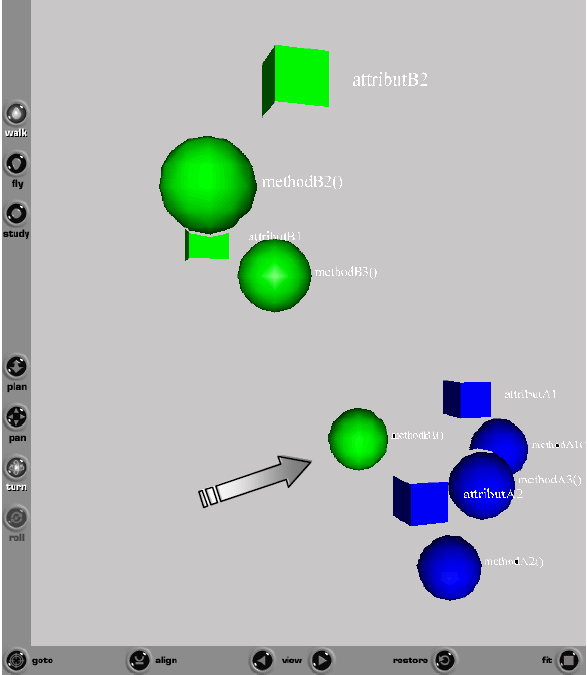
\includegraphics[width=0.75\textwidth]{img/metricsbasedrefactoring.png}
  \caption{Motivates the refactoring move method}
  \label{fig:MetricsBasedRefactoring}
\end{figure}

%\subsubsection{Distance based cohesion on refactoring operations}
In order to make an automated approach to identify "bad smells" it is used a distance based cohesion metric.
With the distance based algorithm it is possible to identify violations to the rule "put together what belongs together". 
There are some refactoring operations that are related to this rule such as, move attribute, extract class, in-line class and move method. 
Regarding the distances a method using only locally defined methods or attributes have a high distance to the methods of other classes. 
Whereas methods that use many attributes and/or methods of other classes have a low distance to them. 
The attributes are compared by the methods that use them. 
For example if an attribute is only used by methods of other classes, that attribute probably should be moved to other class.





\begin{table}[h]
\begin{tabular}{l|l|l|}
\cline{2-3}
                                                 & Example                             &  \\ \hline
\multicolumn{1}{|l|}{Manual Refactoring}         & The user experienced talked in here &  \\ \hline
\multicolumn{1}{|l|}{Semi-Automated Suggestions}  &                                     &  \\ \hline
\multicolumn{1}{|l|}{Semi-Automated Application} &                                     &  \\ \hline
\multicolumn{1}{|l|}{Automated}                  &                                     &  \\ \hline
\end{tabular}
\end{table}



The automated refactoring tool because changes the program and the user might be lost after that. %fix this
The automated refactoring tool when used by unexperienced users is not good because, like the Semi-Automated with suggestions might led the user to do the wrong refactoring.
Because it is an unexperienced user, it is highly probable that the user will blindly follow the suggestions given by the tools. 
This is not what we want because the suggestions might be wrong and it might transform in a wrong program or in a program with less quality than the original one.
The manual refactoring is not desired too, besides being faster to use a tool, because the user is unexperienced is way more safer to use a tool to apply the refactoring operations. 
Unexperienced users tend to do more errors and might forgot some changes that put a correct program incorrect.

The ideal approach is a Semi-Automated tool that applies what the user wants to do. 
This tool is safe because of the preconditions and helps the user to learn how to apply refactoring operations instead of blindly follow them.

